\newpage
\subsection{Caso d'uso UC2: Autenticazione}
\begin{figure}[h] 
	\centering 
	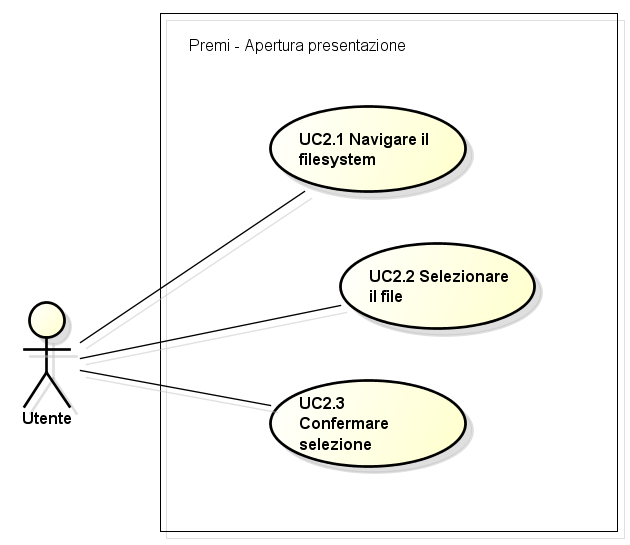
\includegraphics[scale=0.45] {img/UC2.png} 
	\caption{UC2 - Autenticazione} 
\end{figure}

\begin{itemize}
	\item \textbf{Attori:} Utente non autenticato;
	\item \textbf{Scopo e descrizione:} L'utente è già iscritto e vuole avviare la procedura di autenticazione al sito per accedere ai propri file;
	\item \textbf{Precondizione:} L'utente ha selezionato la voce "accedi" presente sul sito;
	\item \textbf{Flusso principale degli eventi:}
	\begin{enumerate}
		\item L'utente inserisce le proprie credenziali [UC2.1];
		\item L'utente conferma l'inserimento dei dati selezionando la voce "login" [UC2.2];
		\item Si può verificare un errore di accesso [UC2.3];
		\item Il sistema controlla i dati inseriti e li accetta [UC2.4];
		\item L'utente viene reindirizzato alla propria pagina personale [UC2.5];
		\item L'utente può recuperare le sue credenziali se le dimentica [UC2.6].
	\end{enumerate}
	\item \textbf{Postcondizione:} Il sistema verifica le credenziali inserite e permette all'utente di accedere alla sua pagina personale.
\end{itemize}

\newpage

\subsection{Caso d'uso UC2.1: Inserimento credenziali}
\begin{figure}[h] 
	\centering 
	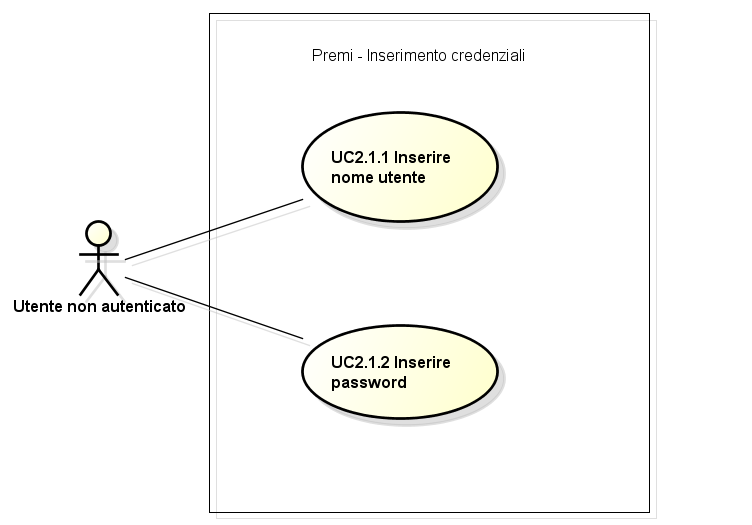
\includegraphics[scale=0.45] {img/UC2.1.png} 
	\caption{UC2.1 - Inserimento credenziali} 
\end{figure}
\begin{itemize}
	\item \textbf{Attori:} Utente non autenticato;
	\item \textbf{Scopo e descrizione:} L'utente inserisce nome utente e password per poter accedere al sito;
	\item \textbf{Precondizione:} L'utente visualizza la schermata di inserimento dei dati richiesti per l'accesso;
	\item \textbf{Flusso principale degli eventi:}
	\begin{enumerate}
		\item L'utente inserisce il proprio nome utente [UC2.1.1];
		\item L'utente inserisce la propria password [UC2.1.2];
	\end{enumerate}
	\item \textbf{Postcondizione:} Tutti i campi richiesti sono stati compilati correttamente.
\end{itemize}

\subsection{Caso d'uso UC2.1.1: Inserire nome utente}
\begin{itemize}
	\item \textbf{Attori:} Utente non autenticato;
	\item \textbf{Scopo e descrizione:} L'utente inserisce il proprio nome utente;
	\item \textbf{Precondizione:} La casella dove inserire il nome utente è vuota;
	\item \textbf{Postcondizione:} La casella è stata compilata con il nome utente inserito dall'utente.
\end{itemize}

\subsection{Caso d'uso UC2.1.2: Inserire password}
\begin{itemize}
	\item \textbf{Attori:} Utente non autenticato;
	\item \textbf{Scopo e descrizione:} L'utente inserisce la propria password;
	\item \textbf{Precondizione:} La casella dove inserire la password è vuota;
	\item \textbf{Postcondizione:} La casella è stata compilata con la password inserita dall'utente.
\end{itemize}

\subsection{Caso d'uso UC2.2: Accesso}
\begin{itemize}
	\item \textbf{Attori:} Utente non autenticato;
	\item \textbf{Scopo e descrizione:} L'utente conferma le credenziali inserite scegliendo di effettuare l'accesso tramite il tasto di login;
	\item \textbf{Precondizione:} Nome utente e password sono stati inseriti;
	\item \textbf{Postcondizione:} Il sistema verifica i dati inseriti.
\end{itemize}

\subsection{Caso d'uso UC2.3: Errore di autenticazione}
\begin{itemize}
	\item \textbf{Attori:} Sistema;
	\item \textbf{Scopo e descrizione:} L'utente ha inserito delle credenziali errate e il sistema blocca l'accesso, riportando l'utente alla schermata di accesso;
	\item \textbf{Precondizione:} Nome utente e password sono stati inseriti in modo errato;
	\item \textbf{Postcondizione:} Il sistema riporta l'utente alla schermata di accesso.
\end{itemize}

\subsection{Caso d'uso UC2.4: Dati inseriti correttamente}
\begin{itemize}
	\item \textbf{Attori:} Sistema;
	\item \textbf{Scopo e descrizione:} Il sistema ha verificato che le credenziali inserite sono corrette;
	\item \textbf{Precondizione:} Nome utente e password sono stati inseriti;
	\item \textbf{Postcondizione:} Il sistema ha verificato che i dati inseriti sono corretti.
\end{itemize}

\subsection{Caso d'uso UC2.5: Reindirizzamento a pagina personale}
\begin{itemize}
	\item \textbf{Attori:} Sistema;
	\item \textbf{Scopo e descrizione:} Il sistema dopo aver consentito l'accesso all'utente mostra la sua pagina personale;
	\item \textbf{Precondizione:} Nome utente e password sono stati inseriti correttamente;
	\item \textbf{Postcondizione:} Il sistema mostra la pagina personale dell'utente.
\end{itemize}

\subsection{Caso d'uso UC2.6: Recupero dati}
\begin{figure}[h] 
	\centering 
	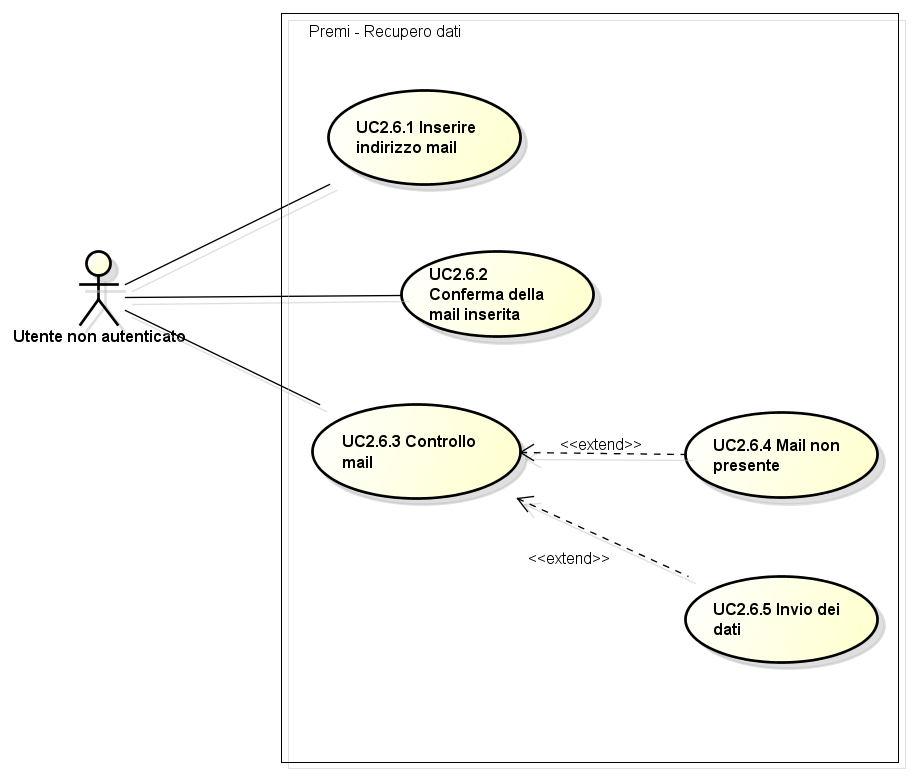
\includegraphics[scale=0.45] {img/UC2.6.png} 
	\caption{UC2.6 - Recupero dati} 
\end{figure}
\begin{itemize}
	\item \textbf{Attori:} Utente non autenticato;
	\item \textbf{Scopo e descrizione:} L'utente non ricorda più le sue credenziali di accesso e sceglie quindi l'opzione per il recupero di tali dati. Il sistema gestirà la richiesta inviando alla mail dell'utente tutti i suoi dati;
	\item \textbf{Precondizione:} L'utente ha selezionato l'opzione di recupero dei dati;
	\item \textbf{Flusso principale degli eventi:}
	\begin{enumerate}
		\item L'utente inserisce il proprio indirizzo mail [UC2.6.1];
		\item L'utente conferma l'inserimento dell'indirizzo mail [UC2.6.2];
		\item Il sistema controlla la mail inserita [UC2.6.3];
		\item Il sistema non trova la mail nel database e segnala un errore [2.6.4];
		\item Il sistema trova una corrispondenza con la mail indicata e invia i dati [2.6.5].
	\end{enumerate}
	\item \textbf{Postcondizione:} Il sistema ha inviato una mail contenente i dati di accesso relativi all'utente che ne ha fatto richiesta.
\end{itemize}

\subsection{Caso d'uso UC2.6.1: Inserire indirizzo mail}
\begin{itemize}
	\item \textbf{Attori:} Utente non autenticato;
	\item \textbf{Scopo e descrizione:} L'utente inserisce il proprio indirizzo mail nella casella vuota;
	\item \textbf{Precondizione:} La casella dove inserire mail è vuota;
	\item \textbf{Postcondizione:} La casella è stata compilata con la mail inserita dall'utente.
\end{itemize}

\subsection{Caso d'uso UC2.6.2: Conferma della mail inserita}
\begin{itemize}
	\item \textbf{Attori:} Utente non autenticato;
	\item \textbf{Scopo e descrizione:} L'utente conferma la mail inserita in precedenza e invia la richiesta;
	\item \textbf{Precondizione:} L'utente ha inserito un indirizzo mail;
	\item \textbf{Postcondizione:} L'utente ha confermato la mail inserita.
\end{itemize}

\subsection{Caso d'uso UC2.6.3: Controllo mail}
\begin{itemize}
	\item \textbf{Attori:} Sistema;
	\item \textbf{Scopo e descrizione:} Il sistema controlla che la mail inserita dall'utente sia già presente nel database;
	\item \textbf{Precondizione:} L'utente ha confermato l'inserimento del proprio indirizzo mail;
	\item \textbf{Postcondizione:} Il sistema ha controllato che la mail inserita esista nel database.
\end{itemize}

\subsection{Caso d'uso UC2.6.4: Mail non presente}
\begin{itemize}
	\item \textbf{Attori:} Sistema;
	\item \textbf{Scopo e descrizione:} Il sistema non trova la mail nel database e lo segnala all'utente;
	\item \textbf{Precondizione:} Il sistema ha controllato la mail inserita e non ha trovato corrispondenze nel database;
	\item \textbf{Postcondizione:} Il sistema avvisa l'utente che la mail inserita non esiste nel database.
\end{itemize}

\subsection{Caso d'uso UC2.6.5: Invio dei dati}
\begin{itemize}
	\item \textbf{Attori:} Sistema;
	\item \textbf{Scopo e descrizione:} Il sistema ha trovato la mail nel database e invia le credenziali alla mail dell'utente;
	\item \textbf{Precondizione:} Il sistema ha controllato la mail inserita e ha trovato una corrispondenza nel database;
	\item \textbf{Postcondizione:} Il sistema invia le credenziali alla mail indicata all'utente e avvisa l'utente dell'avvenuto invio.
\end{itemize}

\newpage